\section{Розробка підходу до вирішення завдання}

\subsection{Огляд аналогів}
magic table

\subsection{Схема розв’язання}
% TODO: якось не consistently виходить. 
% TODO: Треба чітко розділити визначення capacity та задачу прогнозування як таку. ЗАПИТАТИ
% TODO: переробити перший розділ: частіше згадувати визначення пропускної здатності
% TODO: додати в другий розділ щось, де визначається пропускна здатність
Задача моєї дипломної роботи полягає в визначенні пропускної здатності маркетингового каналу. Для виконання задачі необхідно отримати перспективну інформацію щодо функціонування каналу та проаналізувати її. Схема розв’язання задачі зображена на рисунку \ref{fig:solution_schema}.

Пропонується прогнозувати діяльність маркетингового каналу за допомогою імітаційного моделювання. В перших двох діях на діаграмі активностей формулюються правила ділової гри та формується структура каналу, що дозволяє третьою дією побудувати імітаційну модель. Після того як модель побудована, можна запускати процес імітації (дія №4), який буде генерувати вихідні дані, що будуть проаналізовані: буде визначена пропускна здатність каналу.

% TODO: IDEF0 сюда!

%В даній роботі пропонується вирішувати задачу отримання перспективної інформації щодо функціонування маркетингового каналу за допомогою імітаційного моделювання, а саме: %побудувати мережу Петрі відповідно до структури каналу та автоматизувати ділову гру. 
%Задача:
% TODO: в чому задача: знайти пропускну здатність чи отримати перспективну інформацію? 

%Постановка задачі: розробки софта, моделювання
%1. Сформулювати правила гри
%2. Сформувати структуру каналу
%3. Побудувати імітаційну модель (мережу Петрі) 
%4. Провести імітацію
%5. Проаналізуівати отриману статистику -> визначити пропускну здатність каналу (приділити цьому увагу?)
%6. 
            \begin{stdfigure}
                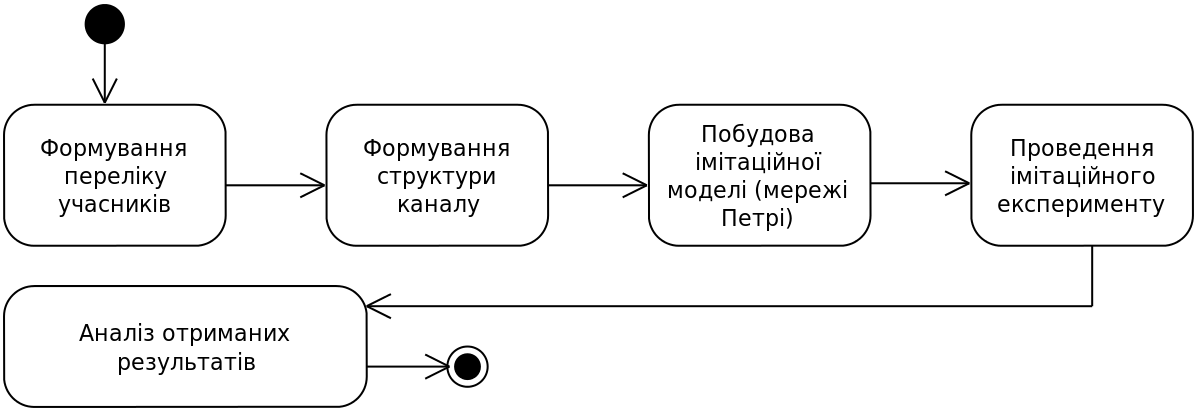
\includegraphics[width=7in]{images/uml_act_solution_schema.png}
                \caption{Схема вирішення задачі в вигляді діграми активностей}
                \label{fig:solution_schema}
            \end{stdfigure}   
% TODO: некрасивая
%\subsection{Теорія ігор}
%Что такое.
%Типы задач, способы описания задач.
%Решение задач.
% TODO: убрать теори игр? Зачем она?

%Деловая игра -- это игра с ненулевой суммой .... 
%Привести задачу одним из способов.
\subsection{Імітаційне моделювання}
\subsubsection{Огляд}
Моделювання --- це процесс побудови моделі для заміни досліджуємого об’єкту з метою дослідження його властивостей, прогнозування поведінки на основі властивостей моделі та характеристик її поведінки\cite{model}.

В залежності від характеру досліджуємих процесів всі види моделювання можуть бути розділені на детерміновані та стохастичні, статичні та динамічні, дискретні, безперервні та дискретно-безперервні. Детерминове модулвання відображає детерміновані процеси, тобто процесі, в яких передбачається відсутність будь-яких випадкових впливів; стохастичне моделювання відображає імовірнісні процеси та події. Статичне моделювання служить для описання поведінки моделі в будь-який момент часу, а динамічне відображає поведінку об’єкту в часі. Дискретне моделювання відображає дискретні процеси, а безперервне -- безперервні процеси\cite{model}.

Виділяють наступні основні методи моделювання\cite{model}:
\begin{longEnumerate}
   \item Математичне моделювання --- процес встановлення відповідності даному реальному об’єкту деякого математичного об’єкту, що називається математичною моделлю, та дослідження цієї моделі, що дозволяює отримувати характеристики об’єкта. 
   \item Аналітичне моделювання. В аналітичному моделюванні процеси записуються в вигляді функціональніх співвідношень та логичніх умов.
   \item Імітаційне моделювання. В цьому виді моделювання алгоритм, що реалізує модель, відтворює процес функціонування системи у часі.
   \item Комбіноване моделювання -- при будуванні комбінованих моделей для деякі складових процесу функціонування використовують аналітичні моделі, де можливо. Для залишившихся використовують імітаційні моделі.
\end{longEnumerate}

Імітаційне моделювання дозволяє досліджувати більш складні системи, ніж аналітичне моделювання. Імітаційна модел може відображать дискретність, нелінійність, недетермінованість та інші якості системи, які неможливо врахувати в аналітичних моделях. Імітаційне моделювання.
% TODO: дописать раздел

\subsubsection{Мережі Петрі}
Що таке імітаційне моделювання?

Навести приклад мережі Петрі, розробленої для каналу для каналу.
% TODO: побудувати модель саме тут?

\subsubsection{Теорія ділових ігор}
	Якісь схеми ігор.



\subsection{Виводи до розділу}
Обосновать выбор.
